% ************************************
\section{Quantum Computing in a Nutshell}
% ************************************

\begin{frame}{Quantum Computing in a Nutshell}

\begin{columns}
 \column{0.6\linewidth}
    \begin{block}{Quantum register}
    $N$-qubit states $\ket{q_1,\dots,q_N}\in\C^{2^N}$
    \end{block}
    
    \vspace{\floatsep}

    \begin{block}{Quantum circuit}
    Unitaries $U_1,\dots,U_L\in \SU(2^N)$
    \end{block}
    
    \vspace{\floatsep}
    
    \begin{block}{Measurement}
    $\Rightarrow$ computational result
    \end{block}
 
 \column{0.4\linewidth}
  \vspace{\floatsep}
    \Qcircuit @C=1em @R=1em {
      \lstick{\ket{q_1}} & \gate{U_1} & \qw & \multigate{1}{U_3} & \meter  \\
      \lstick{\ket{q_2}} & \qw & \multigate{1}{U_2} & \ghost{U_3} & \meter \\
      \lstick{\ket{q_3}} & \qw & \ghost{U_2} & \qw & \meter
    }
 
\end{columns}

\end{frame}

% \begin{frame}{Quantum Speed-Up}
%  
%  \structure{Hope/Expectation:} Many problems can be solved faster on a quantum computer.
%  
%  \begin{columns}
%   \column{0.5\linewidth}
%   \structure{Evidence:} \Eg~Shor's algorithm
%   
%   \column{0.5\linewidth}
%     \begin{figure}
%      \centering
%      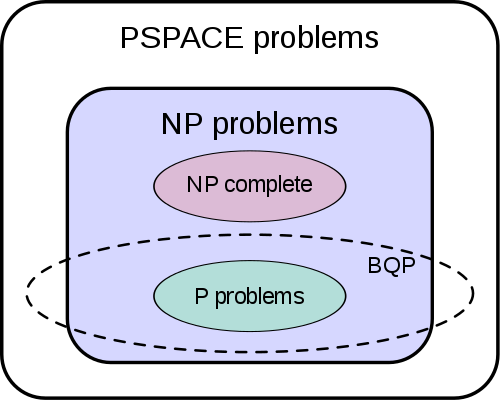
\includegraphics[width=\linewidth]{gfx/BQP_complexity_class_diagram}
%      \caption{\footnotesize Wikipedia/BQP}
%     \end{figure}
%  \end{columns}
%  
% \end{frame}

% \begin{frame}{Quantum Algorithms}
% 
% \structure{Examples:} Grover search algorithm, Shor's factoring algorithm, \dots
% 
% \alert{But: This list is not that long!}
%  
% \end{frame}
